\documentclass[a4paper,twoside,10pt]{report}
\usepackage{geometry}
\usepackage[utf8x]{inputenc}
\usepackage[ngerman]{babel}
\usepackage[german,figure,linesnumbered,lined]{algorithm2e}
\usepackage{tikz}
\usepackage{tkz-fct}
\usepackage{color}
\usepackage{graphics}
\usepackage{graphicx}
\usepackage{amssymb}
\usepackage{amsmath}
\usepackage{listings}
\usepackage{booktabs}
\usepackage{pdfpages}
\usepackage{pgfplots}
\usepackage{float}
\geometry{top=25mm, left=25mm, right=25mm, bottom=30mm}
\lstset{language=C++}
\setlength{\columnsep}{3em}

\begin{document}

\begin{titlepage}
\center
\Large DSEA WS 12-13\large \\[2em]
Dozent:\\Elmar Schömer\\[2em]
Mitschrift von:\\André Groß\\[2em]
Zuletzt Aktualisiert:\\\today\\

\includegraphics[scale=.2]{uni_logo.png}\\[3em]
\Large \textbf{Zusammenfassung:}\\[1em]
\parbox{0.75\textwidth}{\large
Im Mittelpunkt der Veranstaltung stehen Methoden zur Entwicklung (vor allem \mbox{zeit-)} effizienter Algorithmen. Dabei betrachten wir insbesondere solche Datenstrukturen, die eine effiziente Verwaltung von dynamischen Datenmengen ermöglichen. Ein Teil der Algorithmen und Datenstrukturen wird in den Übungen implementiert.\\[.5em]

Mit dem Studium dynamischer Datentypen sowie weiterer Algorithmen schließt die Veranstaltung direkt an Einführung in die Programmierung bzw. Einführung in die Softwareentwicklung an. Allerdings werden nun mathematische Methoden zur Analyse von Algorithmen (Korrektheit und vor allem Aufwand) eingesetzt.\\[.5em]

http://cg.informatik.uni-mainzde/dsea\\
\textbf{Raum:} Mi C02, Mo 03-428\\
\textbf{Abgabe:} Mittwochs 12:00\\
\textbf{Sprache:} Grundsätzlich Java, ggf auch Python
}
\end{titlepage}
\normalsize
\tableofcontents
\twocolumn

\part{Skriptum}
\chapter{Grundlagen}
\section{Divide and Conquer}
Bei einem „teile und herrsche“-Ansatz wird das eigentliche Problem so lange in kleinere und einfachere Teilprobleme zerlegt, bis man diese\linebreak lösen („beherrschen“) kann. Anschließend wird aus diesen Teillösungen eine Lösung für das Gesamtproblem (re-)konstruiert.
\subsubsection{Anwendung}
„Teile und herrsche“ \,ist eines der \,wichtigsten Prinzipien für effiziente Algorithmen. Dabei wird ausgenutzt, dass bei vielen Problemen der Aufwand sinkt, wenn man das Problem in kleinere Teilprobleme zerlegt. Dies lässt sich meist durch Rekursive Programmierung umsetzen, bei der die Teilprobleme wie eigenständige Probleme gleichzeitig parallel oder sequenziell (einzeln nacheinander) behandelt werden, bis sie auf triviale Lö\-sungen zurückgeführt sind oder der \, Restfehler hinreichend klein ist. Bei manchen Algorithmen steckt dabei die Kernidee im Schritt des „Teilens“, während die „Rekombination“ einfach ist (beispielsweise Quicksort). In anderen \linebreak Verfahren (beispielsweise Mergesort) ist das Teilen einfach, während die Rekombination die Kernidee des Algorithmus enthält. In manchen Algorithmen sind beide Schritte komplex.
\footnote[1]{Wikipedia zu D\&C}
\subsection{Arithmetik großer Zahlen}
In der Schule hat man bereits einen oder mehrere Algorithmen gelernt um die Grundrechenarten auf beliebige Zahlen an zu wenden. Hier sollen nun weitere vorgestellt werden.

Als Beispiel für große Arithmetische Operationen kann unter anderem die RSA angeführt werden. Speziell in Programmiersprachen wie C trifft man auf Rundungsprobleme, die abgefangen werden müssen. Hier verlässt man sich oft nicht auf die eingebaute Arithmetik und entwickelt eigene (zuweilen schnellere) Lösungsansätze.

\subsubsection{Addition}
Nehmen wir nun zwei Zahlen und addieren sie wie früher in der Schule\\
\begin{tabular}{lllllllll}
&3&4&2&7&6&5&1\\
+& &$2_1$&$6_1$&$4_1$&4&3&2\\\hline
&3&6&9&2&0&8&3
\end{tabular}\\
%$$3427651+264432=3692083$$
Da Zahlen in verschiedensten Zahlensystemen benutzt und dargestellt werden können, von Binär über Dezimal bis hin zu beliebigen Basen, möch\-ten wir eine gute allgemeingültige\, Darstellung wählen.
Eine beliebige Zahl kann zu jeder Basis folgendermaßen dargestellt werden:
\begin{align*}
A=\sum_{i=0}^{n-1} a_i b^i &:& 0\le a_i<b\\
C=\sum_{i=0}^{n-1} c_i b^i &:& 0\le c_i<b
\end{align*}
Der oben angesprochene Algorithmus hat mit der darauffolgenden Datenstruktur die Laufzeit $$T(n)=c*n$$
\subsubsection{Multiplikation}
Nehemen wir hier nun zwei Binärzahlen: \\[.5em]
\begin{figure}[H]\center\begin{tabular}{l@{ }l@{ }l@{ }l@{ }l@{ }l@{ }l@{ }l@{ }l@{ }l@{ }l@{ }l@{ }l@{ }l@{ }l@{ }l@{ }l}
1&0&1&0&1&1&0&1&0&$\bullet$&1&1&1&1&0&0&1\\
&&&&&&&&A&$\bullet$&&&&&&&C\\
\\
&&1&0&1&0&1&1&0&1&0&.&.&.&.&.&.\\
&+&&1&0&1&0&1&1&0&1&0&.&.&.&.&.\\
&+&&&1&0&1&0&1&1&0&1&0&.&.&.&.\\
&+&&&&1&0&1&0&1&1&0&1&0&.&.&.\\
&+&&&&&0&0&0&0&0&0&0&0&0&.&.\\
&+&&&&&&0&0&0&0&0&0&0&0&0&.\\
&+&&&&&&&1&0&1&0&1&1&0&1&0\\\hline
&&&&&&..&1&1&1&0&0&0&1&0&1&0
\end{tabular}
\caption{Binäre Multiplikation}
\end{figure}
Dieser Algorithmus kann mathematisch folgendermaßen aufgefasst werden:
\begin{align*}
=&AB\\=&\left(\sum_{i=0}^{n-1} a_i b^i\right)\left(\sum_{j=0}^{n-1} c_j b^j\right)\\=&\sum_{i=0}^{n-1}\sum_{j=0}^{n-1}  a_i c_j b^{i+j}
\end{align*}
Die Schulmultiplikation hat eine Laufzeit von\linebreak $T(n)=c*n^2$. Dies bedeutet für große Zahlen, z.B. $$n=10^6 \Rightarrow T(n)=10^{12}$$
Dies kostet uns sehr viel Zeit. Das die Addition schneller geht zeigte uns der Student Karazuba\footnote{Paper von Karazuba und Offman}.
\subsubsection{Erster Ansatz mit D\&C}

Wir haben Zwei Zahlen $A$ und $C$ von welchen wir je die vordere und die Hintere hälfte nehmen. 
\begin{figure}[H]
\center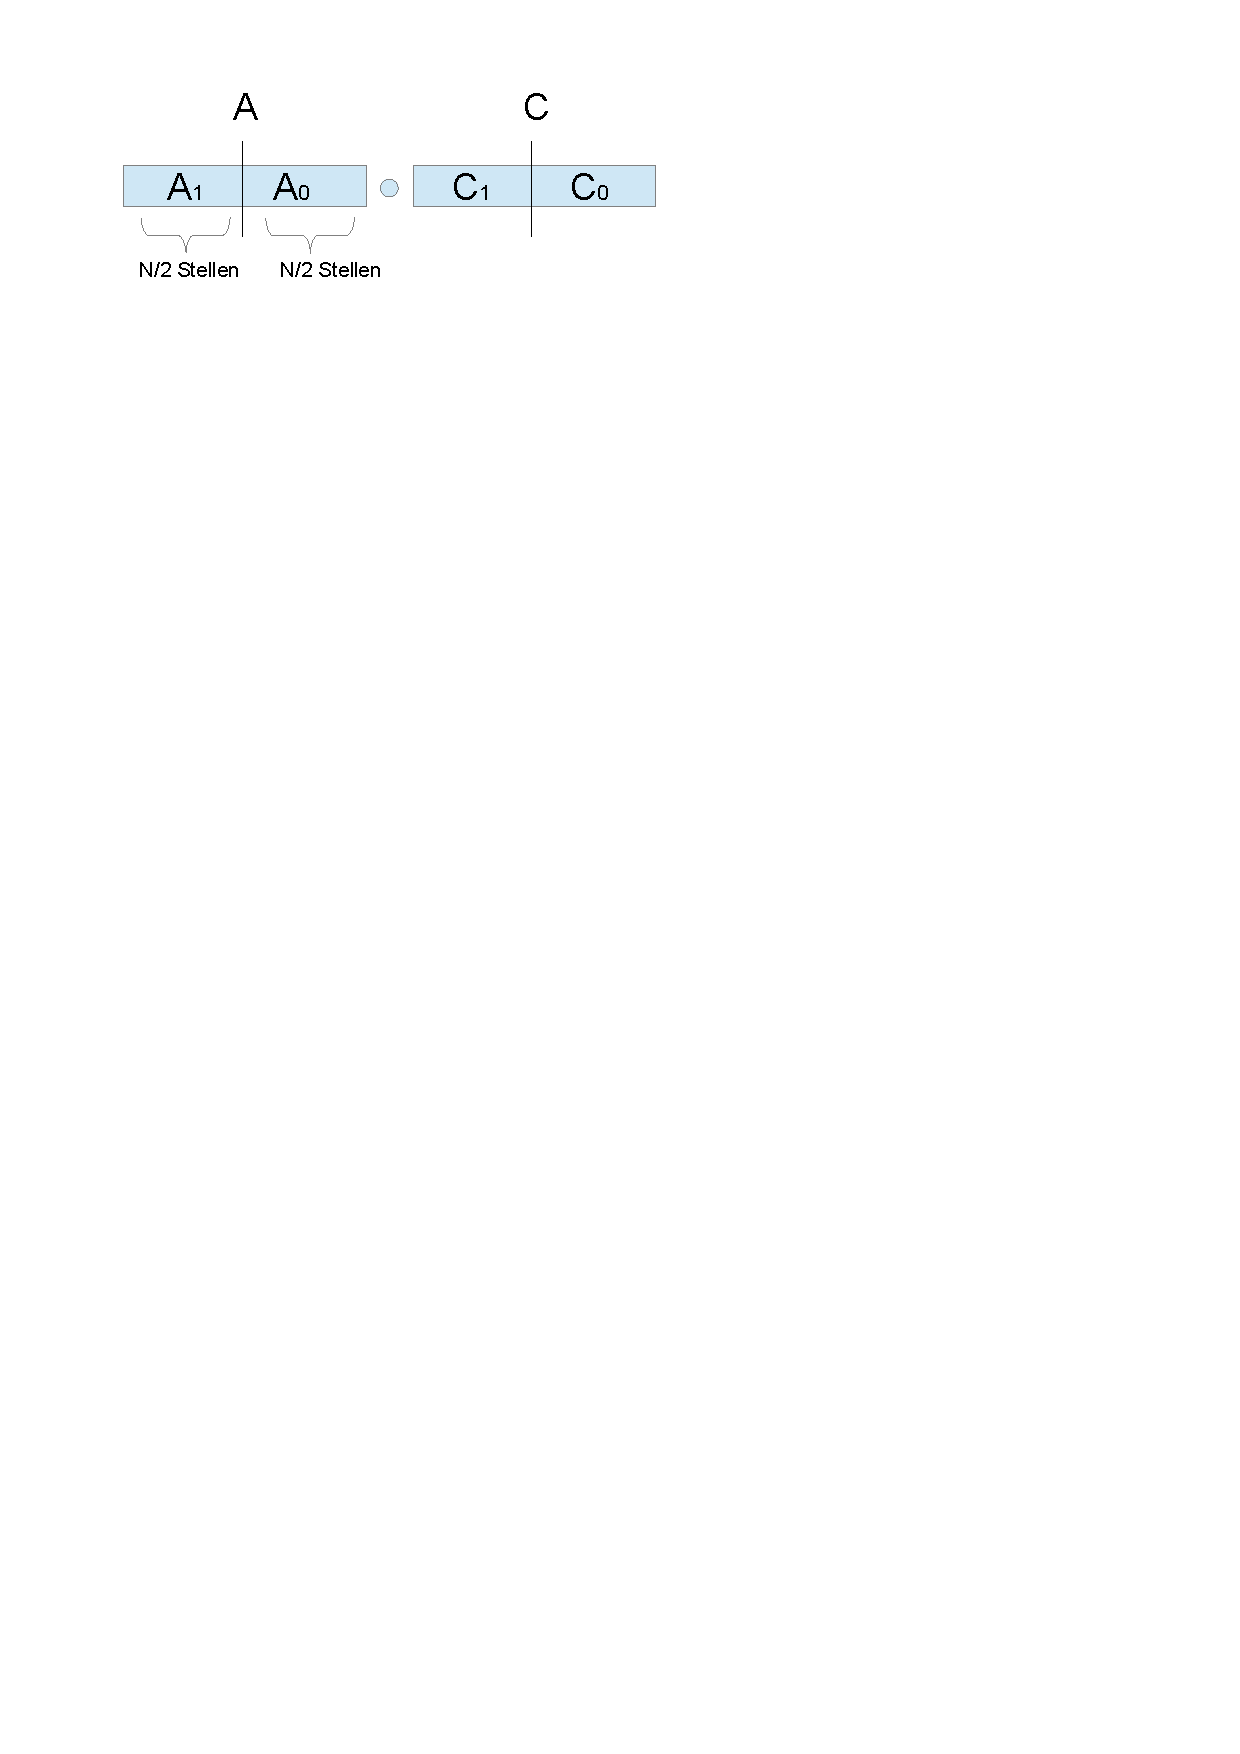
\includegraphics[trim= 2cm 25cm 9.5cm 1.5cm,clip,width=\columnwidth]{DundC.pdf}
\caption{Divide and Conquer bei zwei Feldern}
\end{figure}
Damit ergeben sich folgende Rechenschritte
\begin{align*}
A&=\sum_{i=0}^{n-1} a_i b^i = A_i b^{\frac{n}{2}}+A_0\\
A_0&=\sum_{i=0}^{\frac{n}{2}-1} a_i b^i\\
A_1&=\sum_{i=0}^{\frac{n}{2}-1} a_{i+\frac{n}{2}} b^i\\
\end{align*}
$b^n$ stellt einen binären Shift dar. Wenn wir nun A in zwei Hälften teilen, ist der vordere Teil ($A_1$) um $b^\frac{n}{2}$ voneinander verschoben.
\begin{eqnarray*}
A=123456;&C=987654\\
A\bullet C&\\
A_1=123;&C_1=987\\
A_0=456;&C_2=654\\
A_1b^\frac{n}{2}+A_0=A\\
123000+456&=123456
\end{eqnarray*}
Hier ist der binäre Shift gut zu erkennen. Wie auch die Addition hat der Binärshift linearen \linebreak Aufwand.

Das Produkt $AC$ kann man nun auch folgendermaßen ausdrücken
\begin{align*}
AC&=(A_1b^{\frac{n}{2}}+A_0)(C_1b^{\frac{n}{2}}+C_0)\\
&=A_1C_1b^n+A_1C_0b^{\frac{n}{2}}\\
&\qquad {}+A_0C_1b^\frac{n}{2}+A_0C_0
\end{align*}
Indem das Problem auf diese Art immer weiter vereinfacht wird, überführe ich das quadratische Problem in viele Additionen mit linearem Aufwand.

Betrachten wir uns nun die Laufzeit des Algorithmus. 
\begin{align*}
T(n)&=4T\left(\frac{n}{2}\right)+cn\\
T(1)&=c
\end{align*}
Dies nennt man eine \textbf{Rekursionsgleichung}!

Eine solche R. sagt nur bedingt etwas über die Laufzeit aus. Hierzu muss man diese Gleichung lösen und ggf. mit Induktion o.Ä. lösen.
Bei Betrachtung der Glieder der rekursiven Folge erhalten wir
\begin{align*}
T(n)&=4^kT\left(\frac{n}{2^k}\right)+cn\sum_{i=0}^{k-1}2^i\\
&=4^kT\left(\frac{n}{2^k}\right)+cn\left(2^k-1\right)\\
\mbox{mit}\log_2n:\\
T(n)&=4^{\log_2n}T(1)+cn\left(2^{\log_2n}-1\right)\\
&=n^2c+cn\left(n-1\right)\\
&\le2cn^2
\end{align*}
Wie man hier sieht, hat auch diese Methode einen quadratischen Aufwand. 

\subsection{Karazuba}
Karazuba hatte die Idee, die Zahl der Teilprodukte von vier auf drei zu minimieren.

Dazu stellen wir das D\&C Produkt $AC$ um.
\begin{align*}
AC&=A_0C_1b^{\frac{n}{2}}+A_1C_0b^{\frac{n}{2}}+A_1C_1b^n+A_0C_0\\
&=\left(A_0C_1+A_1C_0\right)b^{\frac{n}{2}}+A_1C_1b^n+A_0C_0\\
&=P_3b^{\frac{n}{2}}+P_2b^n+P_1
\end{align*}
Wenn wir uns nun die drei Produkte einzeln ansehen ist die Vereinfachung schnell zu erkennen
\begin{align*}
P_1&=A_0C_0\\
P_2&=A_1C_1\\
P_3&=A_0C_1+A_1C_0\\
&=(A_1C_1+A_1C_0+A_0B1+A_0B_0)\\
&\qquad {}-A_1C_1-A_0C_0\\
&=\left((A_1+A_0)(C_1+C_0)\right)-P_2-P_1
\end{align*}
denn man sieht, dass man bei $P_3$ nur noch ein Produkt rechnen muss und die anderen beiden Produkte zur Korrektur mittels Multiplikation\linebreak und damit konstantem Aufwand in die Rechnung einfließen.

Bei der Frage an das Auditorium, wie hoch nun die Laufzeit sei, gab es die folgende\\[.5em]
\textbf{Behauptung}
$$T_K(n)=cn^{\log_23}$$
\begin{figure}[h]
\begin{tikzpicture}[scale=.98]
\begin{axis}[legend pos=north west,legend entries={$n^{\log_23}$,$n^2$,$n$}]
\addplot+[no markers,domain=1:10,thick]{x^1.58496};
\addplot+[no markers,domain=1:10,thick]{x^2};
\addplot+[no markers,domain=1:10,thick]{x};
\end{axis}
\end{tikzpicture}
\caption{Laufzeit Multiplikation}
\end{figure}
Hier ist schön zu sehen, um wie viel niedriger der Aufwand im Gegenzug zu $n^2$ ausgefallen ist. Nachfolgend ein kleines Beispiel mit einer\linebreak Größenordnung von 6 für $n$.
\begin{align*}
n&=10^6\\
n^2&=10^{12}\\
n^{\log_23}=n^{1,58\ldots}&\approx10^{9}
\end{align*}

Normalerweise wird erwartet dass der Verlauf eines effizienteren Algorithmuses folgendermaßen verläuft, wobei man gut erkennen kann, dass der effizientere Algorithmus erst ab einem bestimmten n effizienter ist, als der naive Ansatz.
\begin{figure}[H]
\begin{tikzpicture}[scale=.98]
\begin{axis}[legend entries={$n^2$,$n^{\log_23}$}]
\addplot+[no markers] coordinates {(4.61,22) (4.61,1)};
\addplot+[no markers,domain=1:10,thick]{x^2};
\addplot+[no markers,domain=1:10,thick]{(x^1.58496)+10};
\end{axis}
\end{tikzpicture}
\caption{Laufzeit est. Break-even Point}
\end{figure}

Wie verhällt sich nun die Laufzeit für die doppelte Menge an Eingabedaten?
\begin{align*}
\frac{T_S(2n)}{T_S(n)}&=\frac{c(2n)^2}{c(n)^2}&=4\\
\frac{T_K(2n)}{T_K(n)}&=frac{c(2n)^{\log_23}}{c(n)^{\log_23}}&=3
\end{align*}

Gut zu sehen ist, dass sich der Aufwand bei Verdopplung des Naiven vervierfacht und er sich bei K. nur verdreifacht.
\subsection{Schnelle Matrizenmultiplikation nach Strassen}

wir nehmen zwei Matrizen $A,B\in \mathbb R^{n\times n}$ und\linebreak führen auf diesen eine Multiplikation aus.
\begin{align*}C&=AB\\
c_{ij}&=\sum_{k=1}^na_{ik}b_{kj} &1\le i,j \le n\\
\end{align*}
deren Aufwand
$$T(n)=cn^3$$
entspricht.
\[\left(\begin{array}{c@{ }|c@{ }}
A_{1,1} & A_{1,2} \\\hline
A_{1,1} &A_{2,2}
\end{array}\right)\left(\begin{array}{c@{ }|c@{ }}
B_{1,1} & B_{1,2} \\\hline
B_{1,1} &B_{2,2}
\end{array}\right)=\left(\begin{array}{c@{ }|c@{ }}
C_{1,1} & C_{1,2} \\\hline
C_{1,1} &C_{2,2}
\end{array}\right)\]
$$A_{1,1},A_{1,2},A_{2,1},A_{2,2}\in \mathbb R^{\frac{n}{2}\times\frac{n}{2}}$$
\begin{align*}
C_{1,1}&=A_{1,1}B_{1,1}+A_{1,2}B_{2,1}\\
C_{1,2}&=\ldots\\
&\vdots\\
C_{2,2}&=
\end{align*}
Der Aufwand ist hier nun
\begin{align*}T(n)&=8T\left(\frac{n}{2}\right)+cn^2\\
T(1)&=c
\end{align*}
Wenn man diese Rekursionsgleichung löst erhält man für den Aufwand $$T(n)=c^3$$
Hier kommt nun wieder Karazubas Idee ins Spiel den Aufwand von acht zu sieben zu minimieren.

Dies geschieht folgendermaßen:\\
Hab ich keine Lust zu...\\
Daraus folgt
$$\Rightarrow T(n)=7T\left(\frac{n}{2}\right)+cn^2$$
Die Lösung hiervon, werden wir nun mit Hilfe des Mastertheorems ausrechnen, welches wir uns nach der Zusammenfassung herleiten wollen.
\section{Master Theorem}
Wir wollen nun einen Ansatz liefern um im allgemeinen Rekursionsgleichungen lösen.
Dazu betrachten wir uns Probleme der Größe $\frac{n}{b}$, welche man als Teilprobleme eines Problems $T(n)$ auffassen kann.
Die Laufzeit solcher Probleme ist $T\left(\frac{n}{b}\right)$.
Mit der Anzahl an Teilproblemen und der Betrachtung der konstanten Anteile erhalten wir allgemein für Rekursionsgleichungen die Form
\begin{align*}
T(n)&=aT\left(\frac{n}{b}\right)+cn^\alpha\\
T(1)&=c
\end{align*}
für $T\left(\frac{n}{b}\right)$ folgt
\begin{align*}
T\left(\frac{n}{b}\right)&=aT\left(\frac{n}{b^2}\right)+c\left(\frac{n}{b}\right)^\alpha\\
T\left(\frac{n}{b^2}\right)&=aT\left(\frac{n}{b^3}\right)+c\left(\frac{n}{b^2}\right)^\alpha
\end{align*}
damit ergibt sich für $T(n)$
\begin{align*}
T(n)&=a(aT\left(\frac{n}{b^2}\right)+c\left(\frac{n}{b}\right)^\alpha)+cn^\alpha\\
&=a^2T\left(\frac{n}{b^2}\right)+ac\left(\frac{n}{b}\right)^\alpha+cn^\alpha\\
&\vdots&\\
&=a^kT\left(\frac{n}{b^k}\right)+cn^\alpha\sum_{i=0}^{k-1}\left(\frac{a}{b^\alpha}\right)^i
\end{align*}
Die Rekursion bricht ab, wenn
$$\frac{n}{b^k}=1\Rightarrow k=\log_bn$$
$$n=b^k$$
Um die Lösung zu ermitteln müssen wir uns die möglichen Lösungen Betrachten.\\[.5em]
\fbox{\parbox{.95\columnwidth}{
Exkurs Geometrische Reihe:
\begin{align*}
\sum_{i=0}^{\infty}x^i&=\frac{1}{1-x}\, , \, \mbox{für} |x|<1\\
\sum_{i=0}^{k-1}x^i&=\frac{x^k-1}{x-1}\, , \, \mbox{für} x\neq1
\end{align*}
}}\\[.5em]
{\fbox{\parbox{.95\columnwidth}{Umschreiben der Potenzen:
\begin{align*}
a&=b^{\log_ba}\\
a^{\log_bn}&=\left(b^{\log_ba}\right)^{\log_bn}\\
&=b^{\log_ba\log_bn}\\
&=\left( b^{\log_bn}\right)^{\log_ba}\\
&=n^{\log_ba}
\end{align*}
}}\\[.5em]
\begin{itemize}
\item[\textbf{1. Fall}]$\frac{a}{b^\alpha}<1\Leftrightarrow a<b^\alpha \Leftrightarrow \alpha < \log_ba$
\begin{align*}
T(n)&=a^{\log_bn}T(1)+cn^\alpha\frac{1}{1-\left(\frac{a}{b^\alpha}\right)}\\
&= n^{\log_ba}c+c'n^\alpha\\
&\le c''n^\alpha \,,\,\, \mbox{für hinreichend große n}
\end{align*}
\item[\textbf{2. Fall}]$\frac{a}{b^\alpha}>1$
\begin{align*}
T(n)&=cn^{\log_ba}T(1)+cn^\alpha\frac{\left(\frac{a}{b^\alpha}\right)^{\log_bn}-1}{\frac{a}{b^\alpha}-1}\\
&=cn^{\log_ba}+c'n^\alpha\frac{n^{log_ba}}{n^\alpha}\\
&\le  c''n^{\log_ba}
\end{align*}
Karazuba:
\begin{align*}&&a=3,b=2,\alpha=1\\&&\Rightarrow T_K(n)=cn^{\log_23}\end{align*}
Strassen:
\begin{align*}&&a=7,b=2,\alpha=2\\&&\Rightarrow T_S(n)=cn^{\log_27}\end{align*}
\item[\textbf{3. Fall}]$\frac{a}{b^\alpha}=1 \Rightarrow \alpha = \log_ba$
\begin{align*}
T(n)&=cn^{\log_ba}+cn^\alpha\log_bn\\
T(n)&\le n''n^{\log_ba}\log_bn
\end{align*}
\begin{align*}
&&a=2,b=2,\alpha=1\\
&&\Rightarrow T(n)=cn\log n
\end{align*}
\end{itemize}
Mergesort
\begin{align*}
T(n)&=\left\{\begin{array}{ll}
c&\mbox{für }\,n=1\\
2T(\frac{n}{2})+cn&\mbox{für }\,n\neq1
\end{array}\right.\\
\mbox{mit}\\
T(n)&=aT(\frac{n}{b}+cn^\alpha)\\
&\Rightarrow a=1,b=2,\alpha=1\\
&\Rightarrow \mbox{3. Fall}\\
&\log_ba=\alpha\\
T(n)&=c'n\log_2n
\end{align*}
z.B. binäre Suche
\begin{align*}
T(n)&=\left\{\begin{array}{ll}
c&\mbox{für }\,n=1\\
T(\frac{n}{2})+c&\mbox{für }\,n\neq1
\end{array}\right.\\
&\Rightarrow a=1,b=2,\alpha=0\\
&\Rightarrow\mbox{3. Fall}\\
& \log_21=0\\
T(n)&=c'\log_2n
\end{align*}
\subsection{Erweiterung des Theorems}
$$f(n)=\left\{\begin{array}{ll}c&\mbox{für }\,n=1\\af(\frac{n}{b})+cn^\alpha&\mbox{sonst}\end{array}\right.$$
\begin{itemize}
\item[1. Fall]$\alpha<\log_ba\Rightarrow f(n)\in\mathcal O(n^{\log_ba})$
\item[2. Fall]$\alpha>\log_ba\Rightarrow f(n)\in\mathcal O(n^{\alpha})$
\item[3. Fall]$\alpha=\log_ba\Rightarrow f(n)\in\mathcal O(n^\alpha\log_2n)$
\end{itemize}
\fbox{\parbox{\columnwidth}{Umschreiben der Potenzen:\small
\begin{align*}
\log_bn\in\mathcal O (\log_en)\\
\log_bn=\frac{\log_en}{\log_eb}
\end{align*}
}}

\section{Akra Bazzi- Theorem \, \, (1998)}
\begin{align*}
f(x)=\left\{\begin{array}{ll}
h(x)&\mbox{ für }1\le  x\le x_0\\
af(\frac{x}{b})+g(x)&\mbox{ für }x>x_0
\end{array}\right.
\end{align*}
\fbox{\parbox{\columnwidth}{Verallgemeinerte Form:
\begin{align*}
\sum_{i=1}^m a_if\left(\frac{x}{b_i}\right)+g(nx)\,\mbox{ für }\, x>x_0
\end{align*}
}}\\[.5em]
\[a>0,b>1,g:\mathbb R^+\rightarrow\mathbb R^+\]
\small
\begin{align*}
&\exists d_1,d_2>0: d_1\le h(x)\le d_2\mbox{ für }1\le x\le x_0\\
&\exists c_1,c_2>0:c_1g(x)\le g(u)\le c_2g(x)\mbox{ für }x-\frac{x}{b}\le u \le x 
\end{align*}
\normalsize
\[f(x)\in\theta(x^p(1+\int_1^x\frac{g(u)}{u^{p+1}}du))\]
mit $p=\log_ba,b^p=a$\\
Beweis (Idee):
\begin{align*}
f(x)&=af(\frac{x}{b})+g(x)\\
f(\frac{x}{b}&=af(\frac{x}{b^2})+g(\frac{x}{b})\\
&\vdots\\
f(x)&=a^kf(\frac{x}{b^k}+\sum_{i=0}^{k-1}a^ig(\frac{x}{b^i})\\
\end{align*}
bis $\frac{x}{b^k}=1\Rightarrow k=\log_bx$\\[.5em]
\fbox{\parbox{\columnwidth}{Beispiel:
\[H_n=\sum_{i=1}^n\frac{1}{i}\approx \int_1^n\frac{1}{x}dx\approx\ln n\]
\center
\begin{tikzpicture}[scale=0.66]
\begin{axis}[legend entries={$\int_1^x\frac{1}{x}$,$\frac{1}{x}$}]
\addplot+[area legend,no markers,fill=blue,domain=1:10]{1/x} \closedcycle;
\addplot+[no markers,thick,domain=0.7:10.5,samples=200]{1/x};
\end{axis}
\end{tikzpicture}
}}
\[\sum_{i=0}^{k-1}a^ig(\frac{x}{b^i})\approx \int_0^{k-1}a^ig(\frac{x}{b^i})di\]
\fbox{\parbox{\columnwidth}{Substitution:
\begin{align*}
u&=\frac{x}{b^i}=cb^{-i}\\
\frac{du}{di}&=-\ln b x b^{-i}\\&=-\ln b u\\
di&=-\frac{1}{\ln b u}du
\end{align*}
}}\\[.5em]
\begin{align*}
\Rightarrow\,&=-\frac{1}{\ln b}\int a^ig(u)\frac{1}{u}du\\
&=\frac{1}{\ln b}\int_b^x(\frac{x}{u})^pg(u)\frac{1}{u}du\\
&=\frac{1x^p}{\ln b}\int_b^x\frac{g(u)}{u^{p+1}}du
\end{align*}
mit
\begin{align*}
&i=\log_b\frac{x}{u}\\
&a^i=b^{\log_ba\log_b\frac{x}{u}}=(\frac{x}{u})^{\log_ba}=(\frac{x}{u})^p\\
&i=k-1\Rightarrow u=xb^{-k+1}=(\frac{x}{b^k})b
\end{align*}

\subsection{Anwendung von Akra Bazzi}
$$T(n)=2T(\frac{n}{2})+n\log n$$
$$g(n)=n\log n$$
$$T(n)=\theta (n^1(1+\int_1^n\frac{u\log u}{u^2}du))$$
$$p=\log_ba=1$$
$$\int_1^n\frac{\ln u}{u}du=[\ln^2u]_1^n=\frac{1}{2}\ln^2n$$
$$T(n)=\theta(n(1+\log^2n))=\theta(n\log^2n)$$

\section{Landau-Symbole}
$$f,g:\mathbb N \rightarrow\mathbb N$$
$$f(n)\in \mathcal O(g(n)):\Leftrightarrow\exists c>0\exists n_0\forall n>n_0:f(n)\leq cg(n)$$
$$\Leftrightarrow \limsup_{n\rightarrow\infty}\frac{f(n)}{g(n)}<\infty$$
\textbf{In Worten} " f wächst nicht schneller als g"\\
z.B. $$f(n)=4n^3+6n^2-7n+9\in\mathcal O(n^3)$$
$$\in \Omega(n^3)$$
$$\lim_{n\rightarrow \infty}\frac{f(n)}{g(n)}=\frac{4n^3+6n^2-7n+9}{n^3}=4<\infty$$
$$>0$$
$$f(n)\in\Omega(g(n)):\Leftrightarrow\exists c>0 \exists n_0 \forall n>n_0:f(n)\ge cg(n)$$
$$\Leftrightarrow \liminf_{n\rightarrow\infty}\frac{f(n)}{g(n)}>0$$
Bsp:
$$\mbox{Martin}$$





























\chapter{Sortieren und Ordnen}
\section{Quicksort}
Als Beispiel für einen randomisierten D\&C Algorithmus soll hier Quicksort dienen.

Quicksort ist ein Replace Verfahren, welches den Vorteil hat, \,dass man keinen \,zusätzlichen Speicher zum Sortieren benötigt.

Das Verfahren von Quicksort lässt sich gut an einem Beispiel erklären.
Wir nehmen hierzu ein Feld von Zahlen.
Man versucht beim partionieren mehr Intelligenz in die Sache zu stecken.
Wir suchen uns dazu ein beliebiges Element (Pivot- Element -$P$-) heraus und bilden zwei Mengen von Elementen, eine Menge $X\le P$ und eine Menge $Y\ge P$. Wir bewegen nun das Pivot-Element ans Ende (tauschen) und durchlaufen das Feld mit dem Index $i$ und schreiben die Zahlen kleiner $P$ an den Anfang und die Zahlen Größer $P$ an das Ende.
dann Tauschen wir das Pivot-Element wieder zurück und haben nun zwei Mengen größer, kleiner $P$ im Feld.
\begin{figure}[H]
\begin{verbatim}
partition(int a[],int l,int r){
   int x=a[r];
   int i=l-1;
   for(int j=l;j<r;j++){
      if(a[j]<=x){
         i=i+1;
         swap(a,i,j);
      }
   }
   swap(a,i+1,r);
   return i+1;
}
quicksort(int a[], int l, int r){
   if(l>=r) return;
   int p=partition(a,l,r);
   quicksort(a,l,p-1);
   quicksort(a,p+1,r);
}
\end{verbatim}
\caption{Quicksort}
\end{figure}
\subsection{Laufzeitanalyse}
\textbf{Worst-case}\\
Pivotelement $X$ ist immer das kleinste / größte Element in der betrachteten Teilfolge.
\begin{align*}
T(1)&=0\\
T(n)&=T(n-1)+cn\\
&=T(n-2)+c(n-1+n)\\
&=T(n-3)+c(n-2+n-1+n)\\
&\vdots\\
&=c\sum_{i=1}^n=c\frac{n(n+1)}{2}\in \theta(n^2)\\
\end{align*}
Erinnerung:\\
$$\mathcal X =\mbox{Zufallsvariable}$$
$$E(\mathcal X)=\sum pr(\mathcal X= x_i)x_i$$
z.B. Erwartete Augenzahl bei fairem Würfel
$$E(\mathcal X)=\sum_{i=1}^6\frac{1}{6}i=\frac{1}{6}\frac{67}{2}=3.5$$
z.B. Wieviele Münzwürfe benötigt man bis zum ersten Mal "Kopf" erscheint?
\begin{align*}
E(\mathcal X)&=\sum_{i=1}^\infty \left(\frac{1}{2}\right)^ii\\
E(\mathcal X)&=\frac{1}{2}\sum_{i=1}^\infty\left(\frac{1}{2}\right)^ii=\frac{1}{2}\frac{1}{(1-\frac{1}{2})^2}=\frac{1}{2}\frac{1}{\frac{1}{4}}\\&=2
\end{align*}
\fbox{\parbox{\columnwidth}{\textbf{Nebenrechnung:}\small\begin{align*}\sum_{i=1}^\infty ip^{i-1}&=\frac{d}{dp}\sum_{i=0}^\infty p^i\\
&=\frac{d}{dp}\frac{1}{1-p}=\frac{1}{(1-p)^2}\\&|p|<1\end{align*}}}\\[.5em]
Weiter mit QS:\\
\begin{align*}
T(n) &= \mbox{Erwartungswert}\\
T(n)&=\sum_{i=1}^n\frac{1}{n}\left(T(i-1)+T(n-i)\right)+cn\\
&\in \theta((n+1)ln(n+1)=\theta(n\log n)\\
nT(n)&=\sum_{i=1}^nT(i-1)+\sum_{i=1}^nT(n-i) +cn^2\\
&=2\sum_{i=0}^{n-1}T(i)+cn^2\\
&(n-1)T(n-1)\\
&=2\sum_{i=0}^{n-2}T(i)+c(n-1)^2\end{align*}
\tiny\[nT(n)-(n-1)T(n-1)=2T(n-1)+c(n^2-(n^2-2n+1))\]
\small\begin{align*}
nT(n)&=(n+1)T(n-1)+c'n\\
T(n)&=\frac{n+1}{n}T(n-1)+c'\\
&=\frac{n+1}{n}\left(\frac{n}{n-1}T(n-2)+c'\right)+c'\\
&=\frac{n+1}{n-1}T(n-2)+\frac{n+1}{n}c'+\frac{n+1}{n+1}c'\\
&=\frac{n+1}{n-k}T(n-k-1)+c'(n+1)\sum_{i=n-k+1}^{n+1}\frac{1}{i}\\
&6k:=n-1\\
&=(n+1)T(0)+c'(n+1)\sum_{i=1}^{n+1}\frac{1}{i}
\end{align*}
\normalsize
\section{Selektionsproblem}
Gegeben: Eine Folge von $n$ Elementen (unsortiert)
Gesucht: das $k-t$ kleinste Element
\begin{figure}[H]
\begin{verbatim}
int select(int a[],int l,int r, int k){
   int p= partition(a,l,r);
   if(l+k<p) 
      return select(a,l,p-1,k);
   if(l+k>p) 
      return select(a,p+1,r,k+l-p-1);
   return a[p];
}
\end{verbatim}
\caption{Selection Sort}
\end{figure}
Wir erhalten damit die Rekursionsgleichung
\[T(n)=cn^1+T(\frac{n}{2})\]
Womit wir die Werte$a=1;\, b=2;\,\alpha=1;$ für die Lösung mit dem Mastertheorem erhalten.

\begin{align*}
\Rightarrow& T(n)\in \mathcal O(n)\\
T(n)&=\mbox{Erwartungswert der Laufzeit von select}\\
T(n)&\le cn+\sum_{i=1}^n\frac{1}{n}\max\left(T(i-1),T(n-i)\right)\\
&\le cn+\frac{a}{n}\sum_{1=1}^n\max\left((i-1),(n-i)\right)\\
&\le cn+2\frac{a}{n}\sum_{j=\frac{n}{2}}^{n-1}j\\
&\le cn+2\frac{a}{n}\left(\frac{(n+1)n}{2}-\frac{(\frac{n}{2}-1)\frac{n}{2}}{2}\right)\\
&\le cn+a\left(\frac{3}{4}n-\frac{1}{2}\right)\\
&\le cn+\frac{3}{4}an
\end{align*}
hier fehlt noch was....\\
Mit Gaussformel:
$$\sum_{j=a}^bj=\frac{b(b+1)}{2}- \frac{(a-1)a}{2}$$
\section{Deterministischer Algorithmus für Selektionsproblem}
Das Selektionsproblem sucht den Median von einem Feld indem es das Feld in Blöcke unterteilt
\begin{figure}[H]\center\include{meridian}\caption{Selektionsproblem}\end{figure}
$\frac{3n}{10}$ der Elemente sind$\le M$\\
$$T(n)=cn+T\left(\frac{n}{5}\right)+T\left(\frac{7n}{10}\right)$$
Akra Bazzi Theorem:
\begin{align*}
T(n)&=\sum_{i=1}^ka_iT\left(\frac{n}{b_i}+g(n)\right)\\
\Rightarrow T(n)&= \mathcal O\left( n^p\left(1+\int_1^n\frac{g(u)}{u^{p+1}}du\right)\right)\\
T(n)&=\mathcal O\left(n^p\left(1+\int_1^n\frac{cu}{u^{p+1}}du\right)\right)\\
&=\mathcal O\left(n^p\left(1+\frac{c}{1-p}n^{-p+1}\right)\right)\\
&=\mathcal O(n^p+n^1)=\mathcal O(n)
\end{align*}
\fbox{\parbox{\columnwidth}{Nebenrechnung:\small\begin{align*}&\sum_{i=1}^k\frac{a_i}{b_i^p}=1\\
&g(n)=cn\\
&a_1=a_2=1;\,b_1=5;\, b_2=\frac{10}{7}\\
&\left( \frac{1}{5} \right)^p+ \left( \frac{7}{10} \right)^p=1\\
&p\approx 0,84 \le 1\end{align*}}}\\[.5em]




























\chapter{Einfache Datenstrukturen}
\section{Binäre Bäume}
Wir haben die Zufallsvariablen $\mathcal X_1,\mathcal X_2 $ für die Augenzahl zweier fairer Würfel mit 
\[E(\mathcal X_1)=E(\mathcal X_2)=3,5 \]
\[E(\max(\mathcal X_1,\mathcal X_2))\approx4,47 \]
\[=\sum pr(Z=z) z = \frac{1}{36}1+\frac{3}{36}2+\frac{5}{36}3+\hdots \]
\textbf{Frage:}\\
Was ist die erwartete maximale Tiefe eines naturwüchsigen binären Baumes?

$t_n$ zugehörige Zufallsvariable
\[E(T_n)=\sum_{i=1}^n \frac{1}{n}E(\max(t_{i-1},T_{n-i})+1\]
\fbox{\parbox{\columnwidth}{ Nebenrechnung:\small
\begin{align*}
\max(\mathcal X,\mathcal Y)&\le\log_2(2^x+2^y)\\
E(\max(2^\mathcal X,2^\mathcal Y))&\le E(2^\mathcal X+2^\mathcal Y)=E(2^\mathcal X)+E(2^\mathcal Y )\\
&\mbox{z.B.}\mathcal X=10,\,\mathcal Y=5\\
&\log_2(2^{10}+2^{5})
\end{align*}}}\\[.5em]
neue Zufallsvariable
\[\mathcal X_n=2^{T_n} \,\mbox{expotentielle Tiefe}\]
\begin{align*}
E(\mathcal X_n)&=2\sum_{i=1}^n\frac{1}{n}E(\max(\mathcal X_{i-1},\mathcal X_{n-i}))\\
&\le 2\sum_{i=1}^n\frac{1}{n}(E(\mathcal X_{i-1})+E(\mathcal X_n-i))\\
&=\frac{4}{n}\sum_{j=0}^{n-1}E(\mathcal X_j)
\end{align*}
\fbox{\parbox{\columnwidth}{\textbf{Merke:}\[E(\mathcal X_n)=\frac{4}{n}\sum_{i=0}^{n-1}E(\mathcal X_j)\]}}\\[.5em]


























































%%%%%%%%%%%%%%%%%%%%%%%%%%%%%%%%%%%%%%%%%%%%%%%%%%%%%%%
\part{Die letzte(n) Vorlesung(en)}
\section{AVL \, Bäume \, Wiederholung}

Die Logaritmische Tiefe ist wichtig für die Suchzeit usw.\\
Linker und Rechter Teilbaum dürfen sich für Suche usw. in ihrer Tiefe nur um max. Eins unterscheiden.

\chapter{VL 19.11.2012}
\begin{align*}
f(z) &=(z+c)^p \\
&=\sum_{n=0}^\infty \frac{1}{n!}f^{(n)}(z0)(z-z_0)\\
\mbox{wähle }&z0=0\\
f'(z)&=p(z+c)^{p-1}\\
f''(z)&=p(p-1)(z+c)^{p-2}\\
f^{(n)}(z)&=p(p-1)(p-2)\hdots(p-n+1)(z+c)^{p-n}\mbox{(Taylor)}\\
\mbox{hier fehlt was!}
\end{align*}

\begin{align*}
b_0=1,b_n&=\sum_{i=1}^nb_{i-1}b_{n-i}\\
B(z)&=\sum_{n=0}^\infty b_nz^n\Rightarrow B(z)\frac{1-\sqrt{1-4z}}{2z}\\
\sqrt{1-4z}&=(1-4z)^\frac{1}{2}\\
&=\sum_{n=0}^\infty \left(\begin{array}{c}\frac{1}{2}\\n\end{array}\right)1^{\frac{1}{2}-n}(-4z)^n\\
&=\sum_{n=0}^\infty\begin{array}{c}\frac{1}{2}\\n\end{array}(-4)^nz^n\\
&=1+\sum_{n=0}^\infty \begin{array}{c}\frac{1}{2}\\n\end{array}(-4)^nz^n\\
&=1+\sum_{n=0}^\infty \begin{array}{c}\frac{1}{2}\\n+1\end{array}(-4)^{n+1}z^{n+1}
\end{align*}

hier fehlt auch noch ne Menge...
\[b_n=-\frac{1}{2}\begin{array}{c} \frac{1}{2} \\n+1\end{array}(-4)^{n+1}\]
den rest kann ich nicht lesen....

\section{Bijektion \, zwischen \, Binärbäumen}
\[n=3; c_c=\frac{1}{n+1}\begin{array}{c} 2n\\n\end{array}\Rightarrow c_3=5\]
Graphik

\section{Amortisierte Analyse am Beispiel von 2-5-Bäumen}
a-b-Bäume: Jeder Knoten Des Baumes hat mind a Kinder und Höchstens b Kinder.
Blattorientierte Speicherung der zu verwaltenden Elemente
\begin{figure}[H]
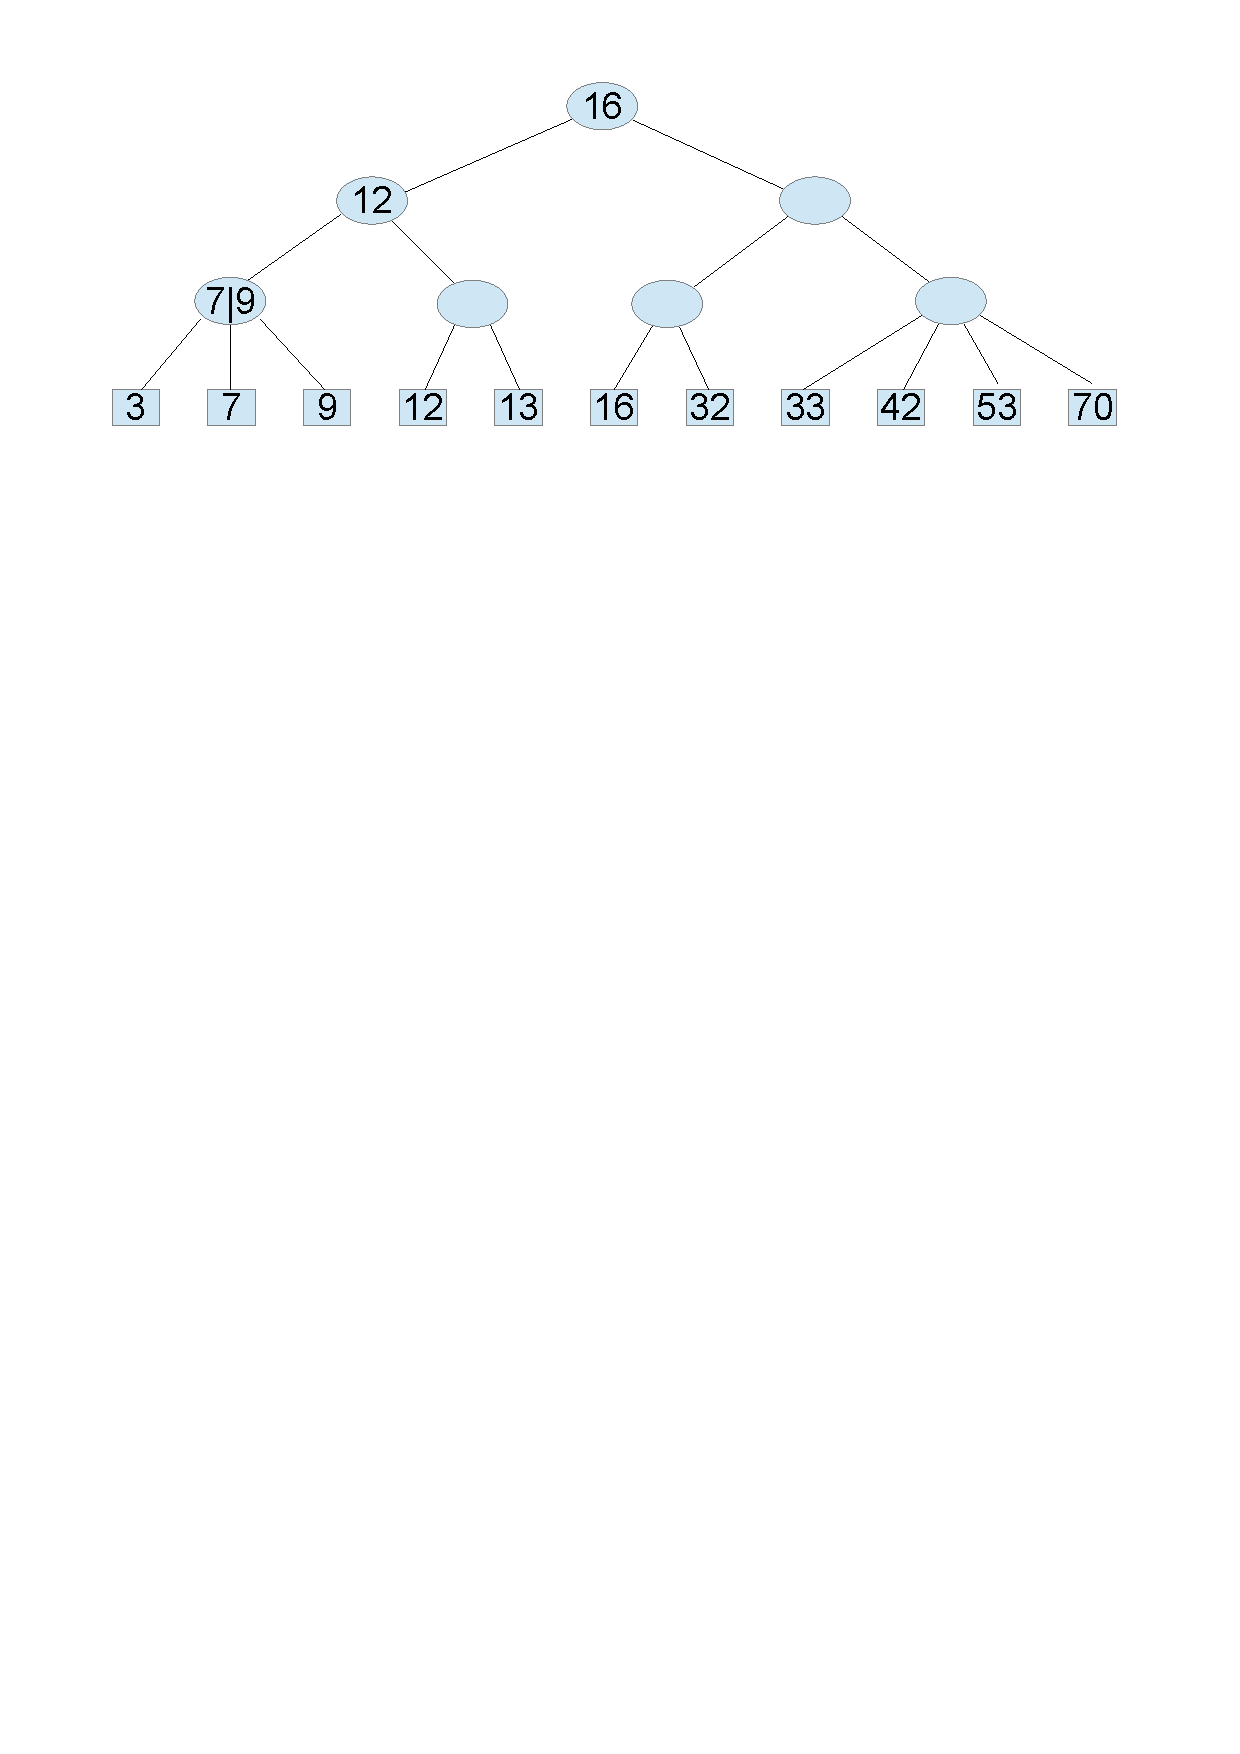
\includegraphics[trim= 1.8cm 20cm 2cm 1.3cm,clip,width=\columnwidth]{aa25baum.pdf}
\caption{2-5-Baum}
\end{figure}
Zahl der Blätter n :
\[2^t\le n\le 5^t\]
\[\log_5n \le t\le  \log_2n\]
\[\Rightarrow t\in \theta (\log n)\]

Strategie zum Einfügen und Löschen von Elementen

\begin{figure}[H]
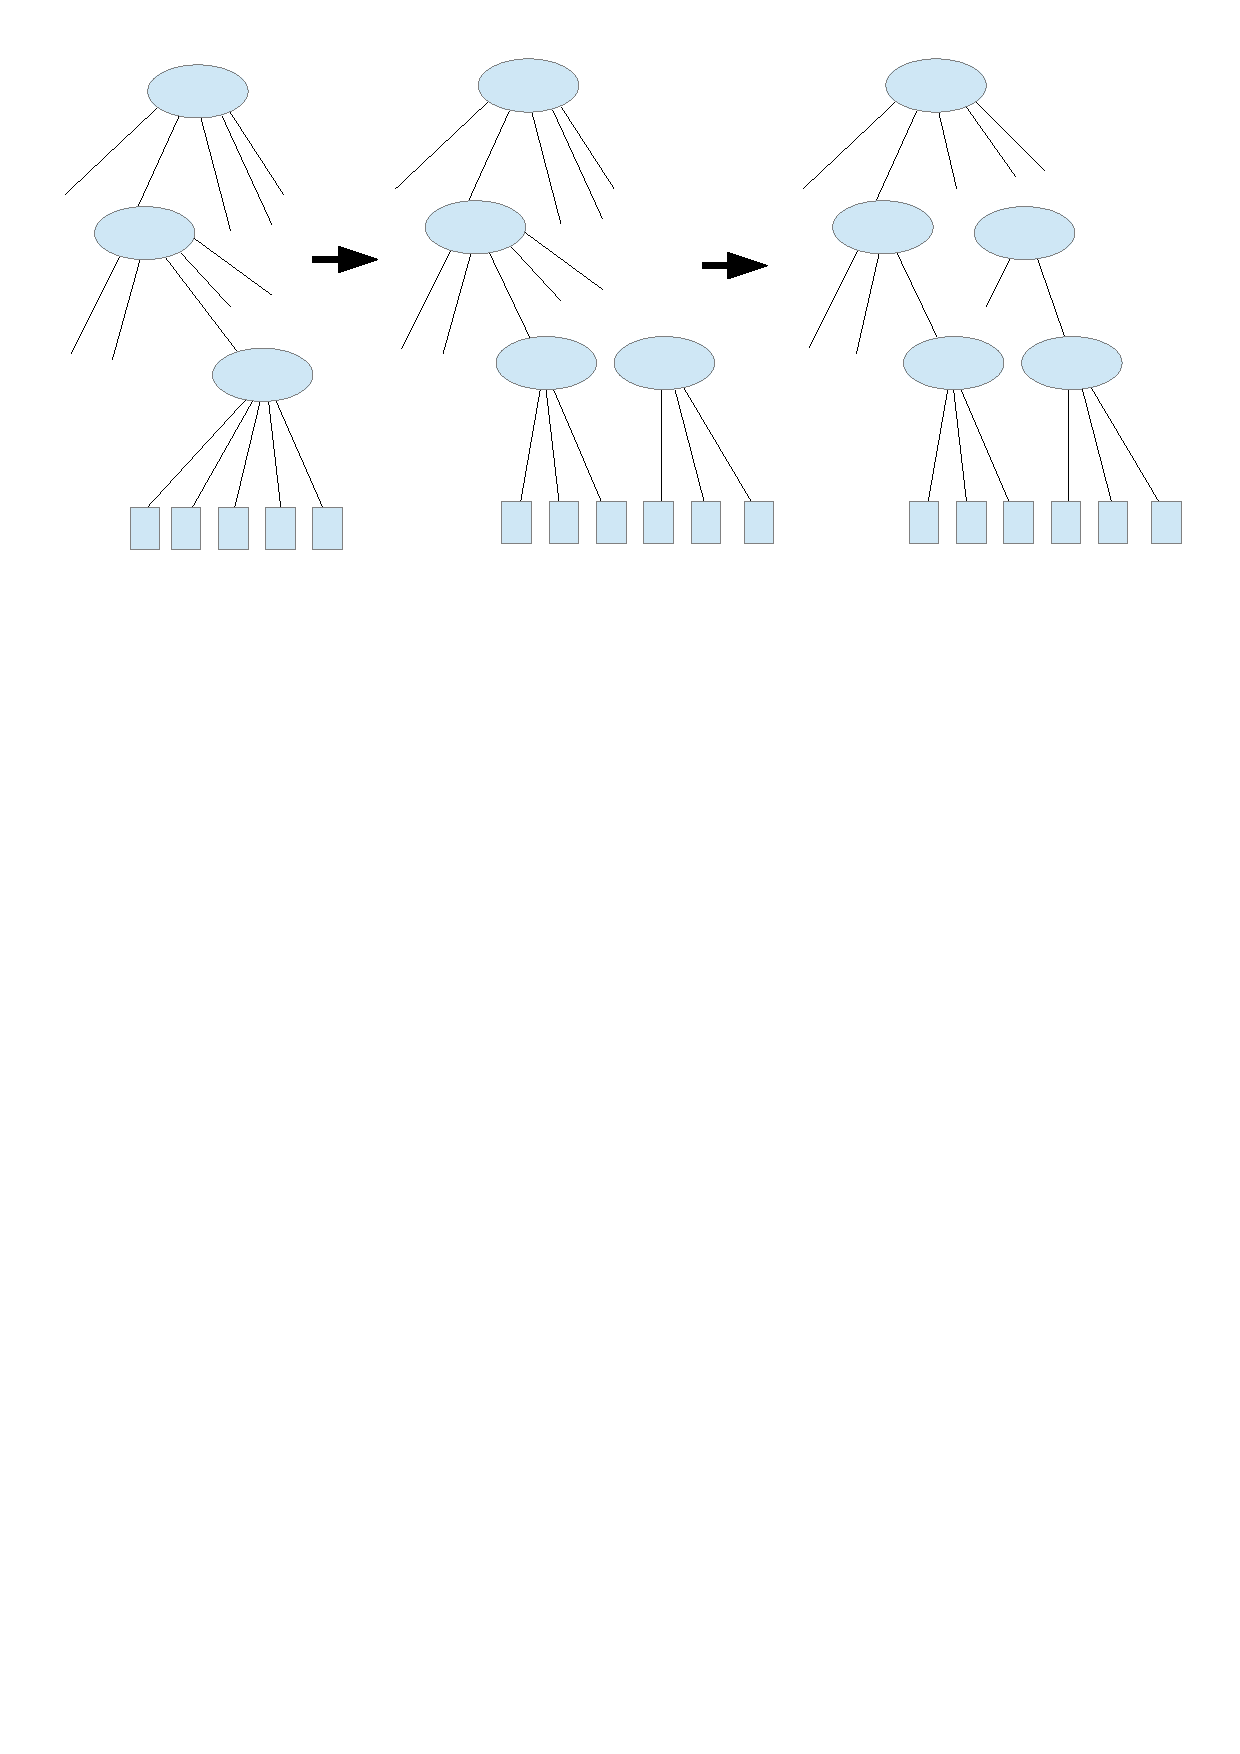
\includegraphics[trim= 1cm 20cm 1cm 1cm,clip,width=\columnwidth]{25bauminsert.pdf}
\caption{Einfügen in 2-5-Baum}
\end{figure}

Beim Löschen von Elementen kann eine Kaskade Von Fusionsoperatoren auf dem Suchpfad notwendig werden. Ggf. Wurzel löschen und Kinder Zusammenlegen.

Laufzeit für Suchen, Einfügen, Löschen $\in \theta(\log n)$

\chapter{VL 21.11}
\section{Amortisierte Analyse am Beispiel des Binärzählers}

\begin{figure}[H]\center
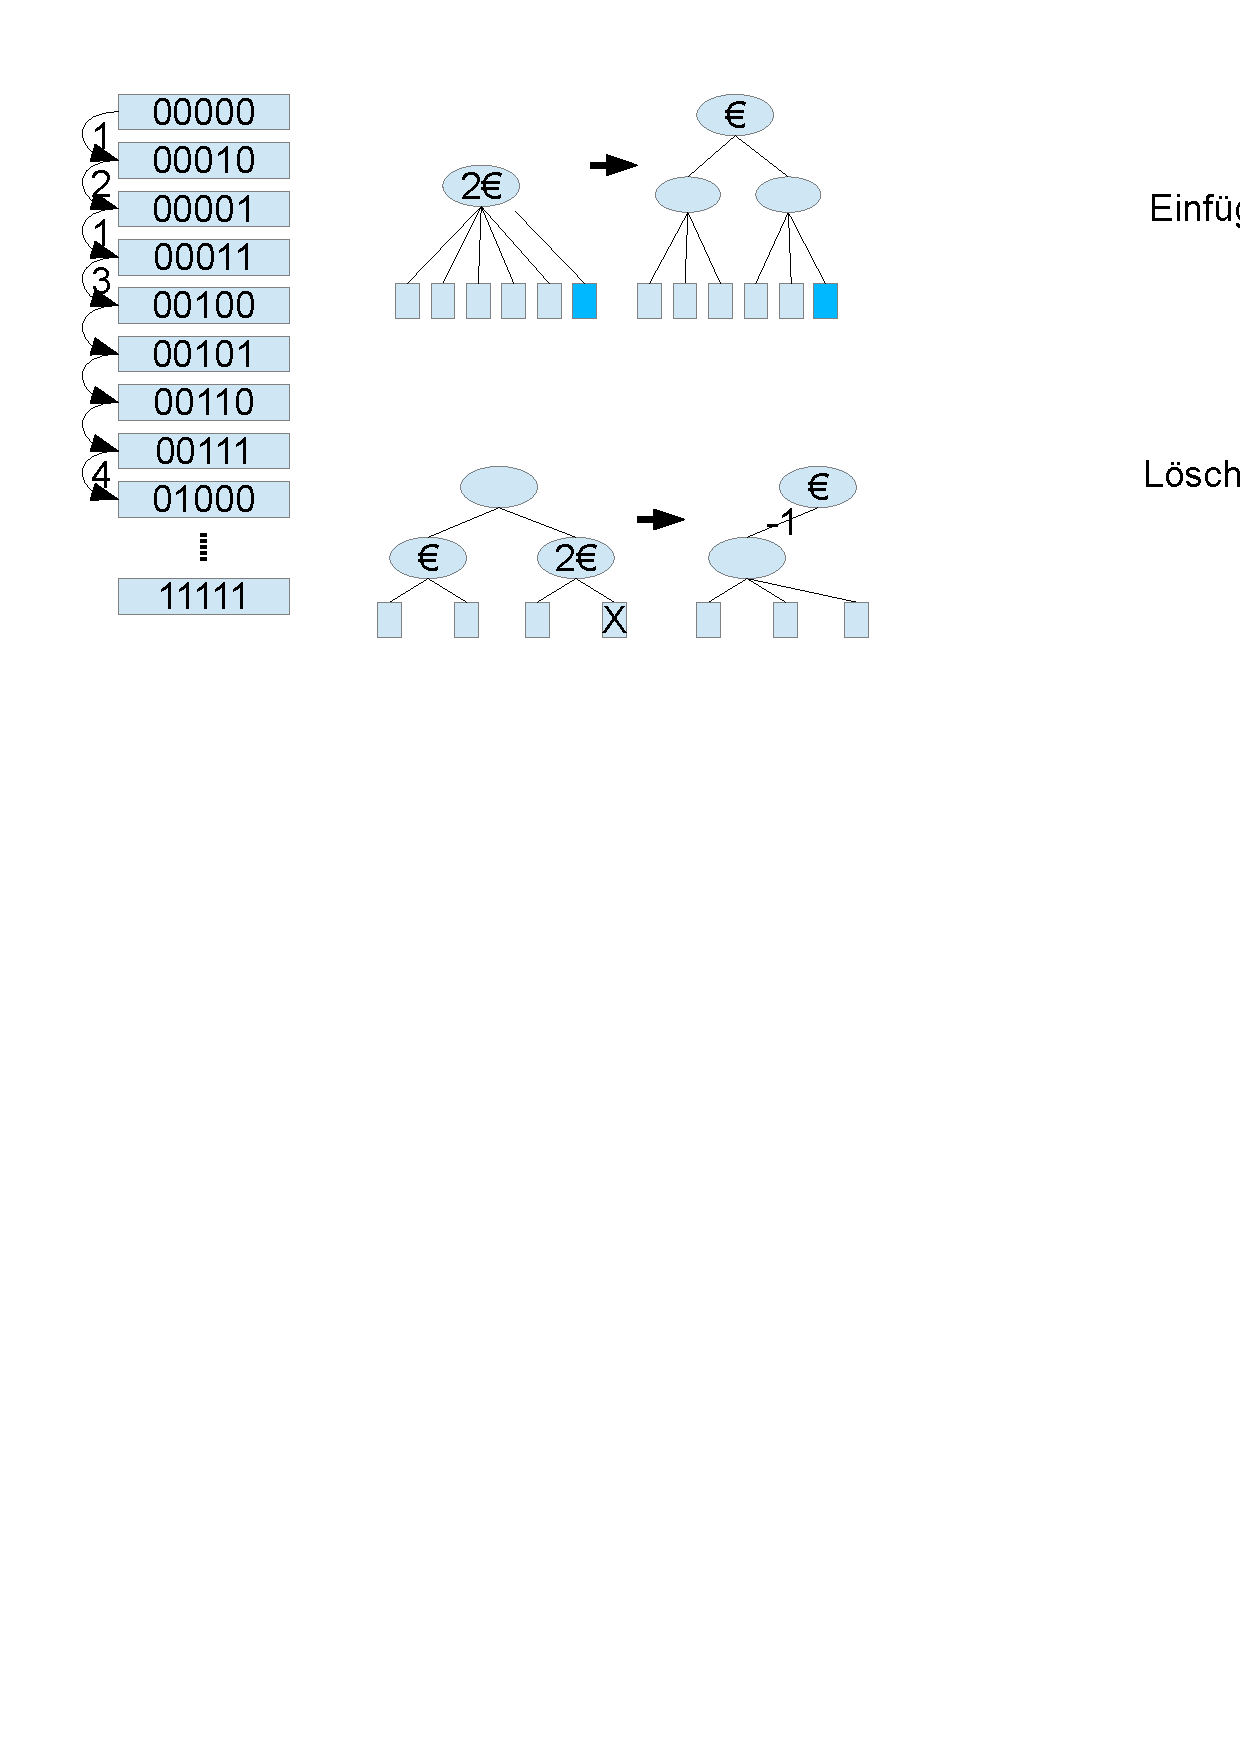
\includegraphics[trim= 1cm 18cm 15cm 1cm,clip,width=0.5\columnwidth]{zaehler.pdf}
\caption{Binärzähler}
\end{figure}

Worst case Kosten einer Inkrement-Operation $\mathcal O(\log_2n)$.

Gesamtkosten für eine Folge von n Inkrement-Operationen (beginnend beim Zählerstand 0)
\begin{align*}
&\frac{n}{2}&\mbox{verursachen Kosten }&1&\mbox{Endung }&0\\
&\frac{n}{4}&\mbox{verursachen Kosten }&2&\mbox{Endung }&01\\
&\frac{n}{8}&\mbox{verursachen Kosten }&3&\mbox{Endung }&011\\
&\frac{n}{16}&\mbox{verursachen Kosten }&4&\mbox{Endung }&0111\\
\end{align*}

Gesamtkosten:\\
\[\le \sum_{i=1}^\infty i\frac{n}{2^i}=n\sum_{i=1}^\infty i\left(\frac{1}{2}\right)^i =2n\]

\fbox{\parbox{\columnwidth}{ Nebenrechnung:\small
\begin{align*}
x\sum_{i=1}^\infty ix^{i-1}&=x\left(\sum_{i=0}^\infty x^i\right)'\\
&=x\left(\frac{1}{1-x}\right)'\\
&=\frac{x}{(1-x)^2}
\end{align*}
}}

\subsection{Kontomethode}
\begin{align*}
Konto(i)&= \mbox{Kontostand vor der i-ten Operation}\\
cost(i)&=\mbox{tatsächliche Kosten der i-ten Operation}\\
\sum_{i=1}^n cost(i)&=\sum_{i=1}^n Konto(i)-Konto(i+1)+a(i)\\
a(i)&=\mbox{ammotisierte Kostender i-ten Operation}\\
\Rightarrow \sum_{i=1}^n cost(i)&=Konto(i)-Konto(n+1)+\sum_{i=1}^n a(i)
\end{align*}

\subsection{amortisierte Analyse der Rekonstruierungskosten für eine Folge von m Einfüge- oder Löschoperationen in einem 2-5-Baum}
Ausgangspunkt: leerer Baum\\
Nicht betrachtet werden die Suchkosten. Wir konzentrieren uns auf die Split- und Fusions-Operationen.\\[.5em]
Kontoführung:\\
\begin{tabular}{rcccccc}
Knotengrad&1&2&3&4&5&6\\
Sparbetrag&2&1&0&0&1&2
\end{tabular}\\[.5em]
Sparplan:\\
$2RE$ pro Einfüge- bzw.Löschoperation\\
$a_i=2$\\
\textbf{Einfügen:}
\begin{figure}[H]\center
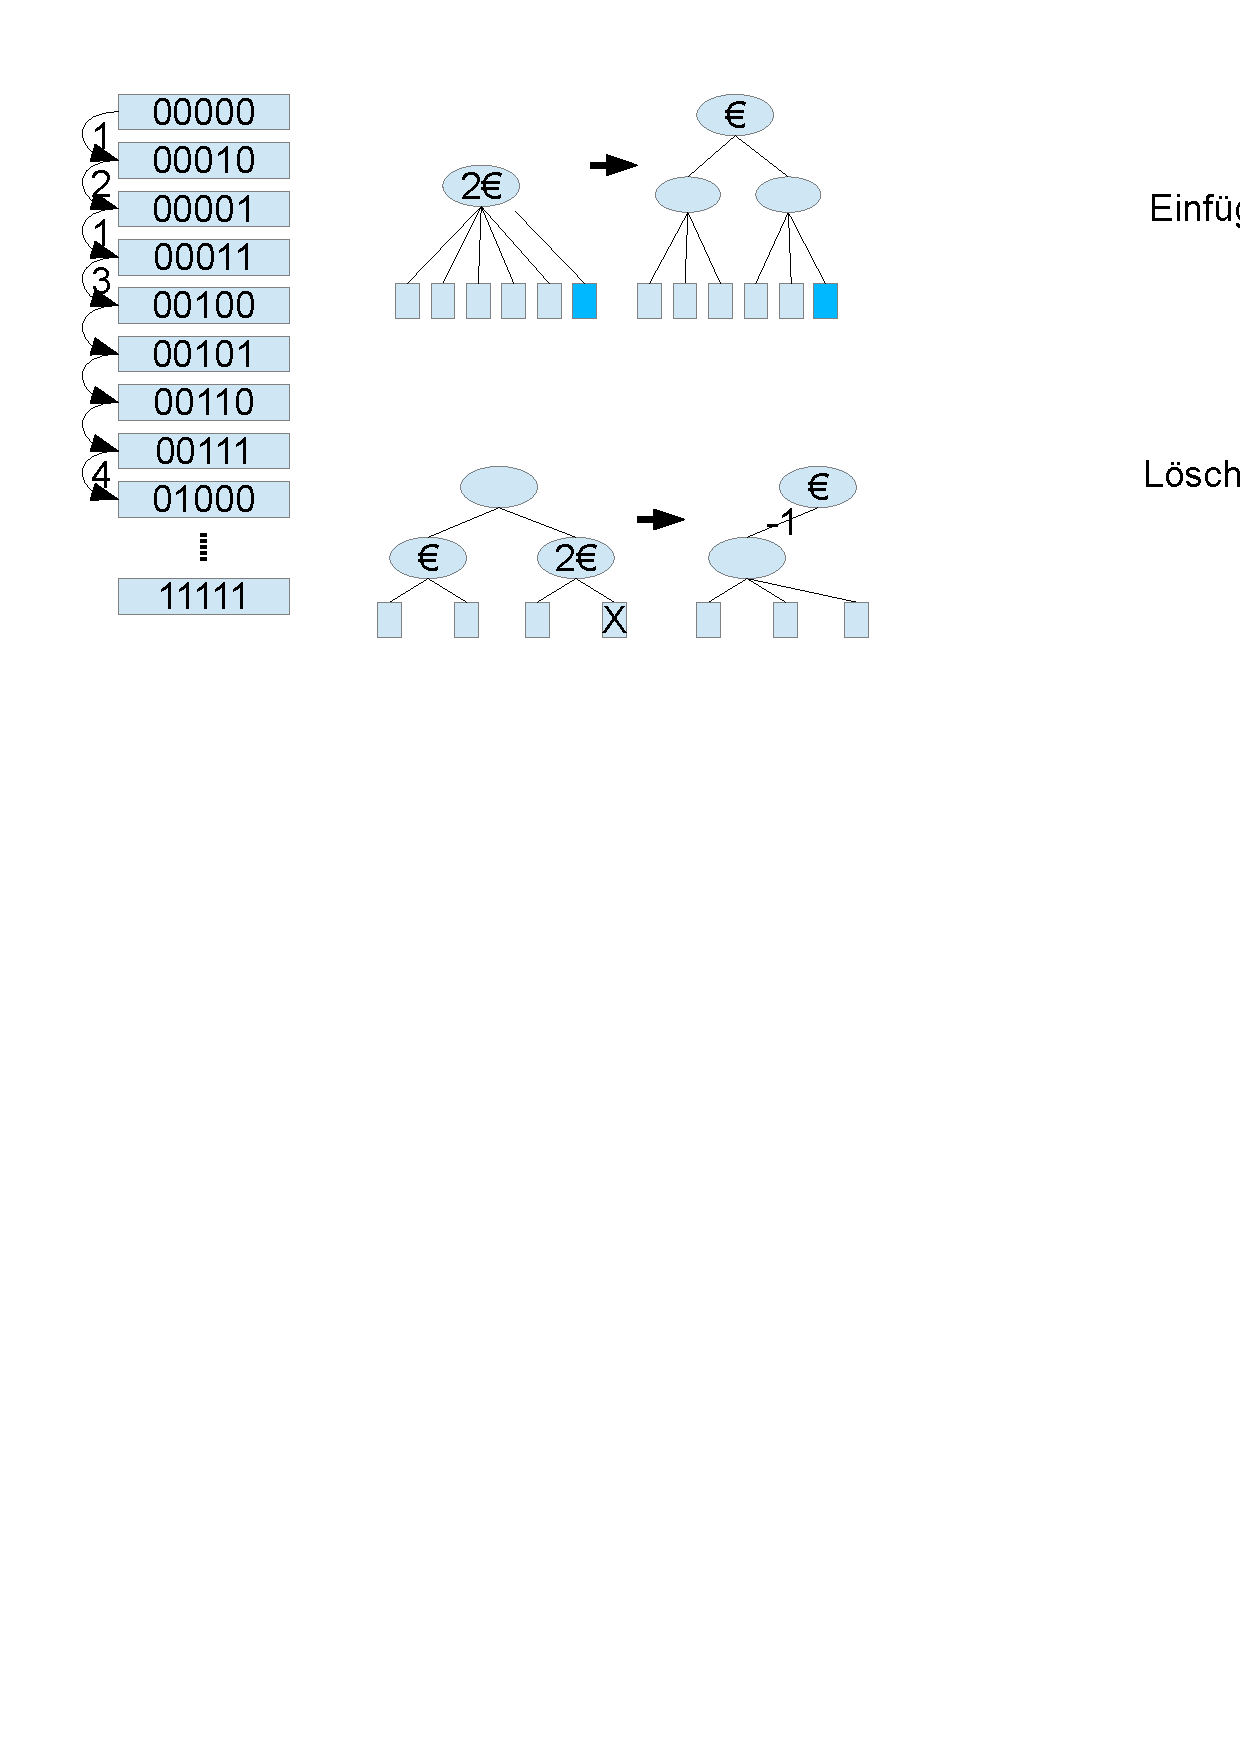
\includegraphics[trim= 6cm 24cm 6cm 1cm,clip,width=\columnwidth]{zaehler.pdf}
\caption{Kosten 2-5-Baum einfügen}
\end{figure}
\textbf{Löschen:}
\begin{figure}[H]\center
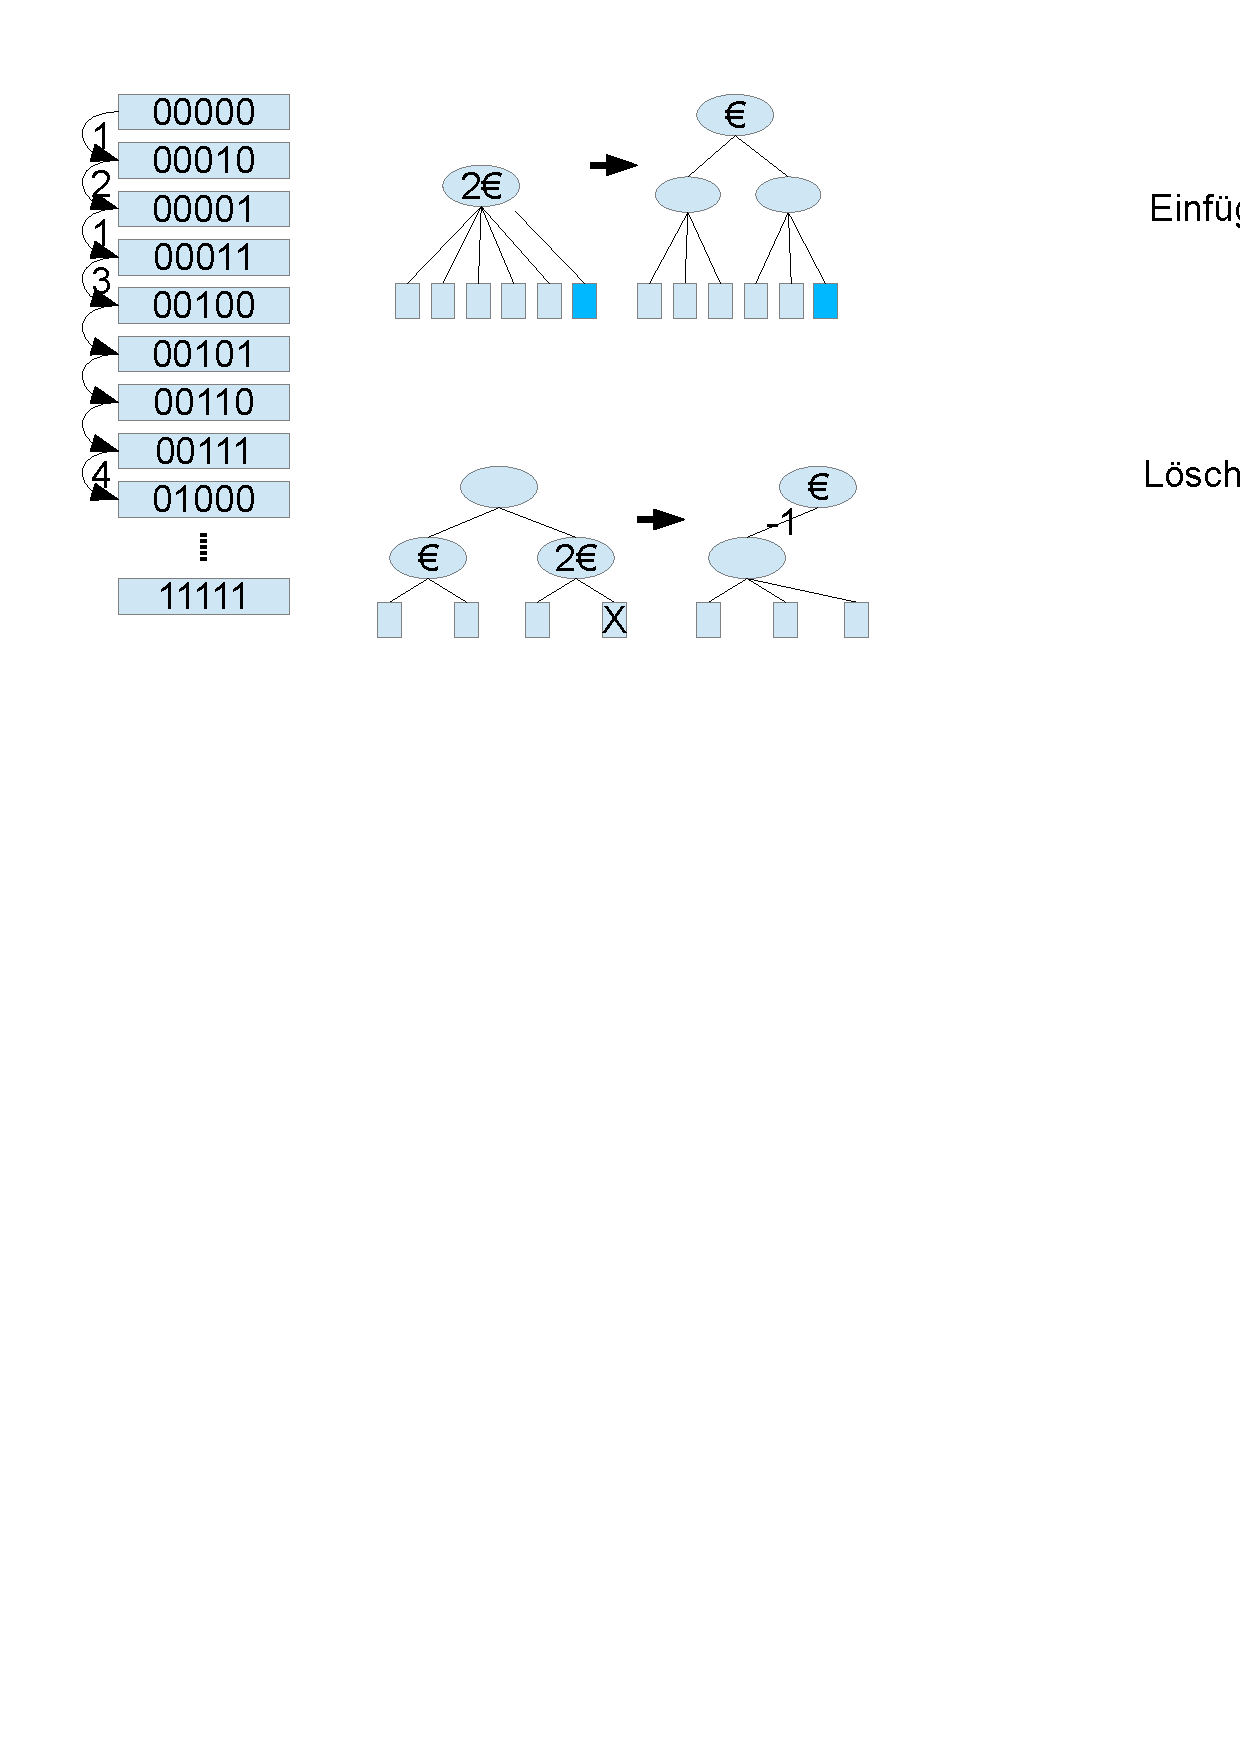
\includegraphics[trim=  6cm 18.5cm 6cm 7cm,clip,width=\columnwidth]{zaehler.pdf}
\caption{Kosten 2-5-Baum Löschen}
\end{figure}

Die m Einfüge- und Löschoperationen auf einem anfangs leeren Baum haben amotisierte Kosten=2.
$\Rightarrow$ Rekonstruierungskosten insgesamt belaufen sich auf $2m$




























\end{document}